% Chapter 1

\chapter{Deep Learning and Tomographic Image Reconstruction} % Main chapter title

\label{Chapter3} % For referencing the chapter elsewhere, use \ref{Chapter1} 

%----------------------------------------------------------------------------------------
The impact of deep learning has been immense over the last few years in the field of medical imaging (\cite{litjens2017survey, greenspan2016guest}). Medical image reconstruction has also benefited hugely from the various advances in neural network architectures \cite{wang2020deep,yedder2021deep,reader2020deep}. In the specific case of \ac{CT} image reconstruction, there has been active interest in sparse-view and low-dose reconstruction scenarios. While with \ac{PET} reconstruction on the other hand, low-dose imaging and total body imaging have been on the forefront. In both cases, obtaining high quality reconstructed images is a challenging task. Many established model-based iterative methods account for the low-dose and sparse-view settings to remove artifacts and noise from the reconstruction (\cite{nuyts1998iterative,Elbakri2002,liu2013total}). However, these methods require the knowledge of noise and artifacts statistics and generally have longer reconstruction times \cite{kim2014combining}. Deep learning-based methods on the other hand are claimed to achieve reconstructed images with quality on par with iterative techniques and in a much shorter time frame \cite{leuschner2021quantitative}. In this work, the focus has been on \ac{CT} and \ac{PET} image reconstruction. 
Image reconstruction corresponds to the task of mapping raw projection data retrieved from the detector to image domain data. As depicted in Fig~\ref{fig:dl}, one can broadly identify three different categories of approaches for the implementation of deep learning within the framework of medical image reconstruction:
\begin{itemize}
	\item[(i)] methods that use deep learning as an image processing step that improves the quality of the raw data and/or the reconstructed image (\cite{gong2018pet, maier2018deep}); 
	\item[(ii)] methods that embed deep-learning image processing techniques in the iterative reconstruction framework to accelerate convergence or to improve image quality (\cite{xie2019generative,kim2018penalized,gong2019iterative});
	\item[(iii)] direct reconstruction with deep learning alone without any use of traditional reconstruction methods  (\cite{whiteley2019direct,zhu2018image,haeggstroem2018deeprec}).
\end{itemize}

\begin{figure}[!htbp]
	\centering
	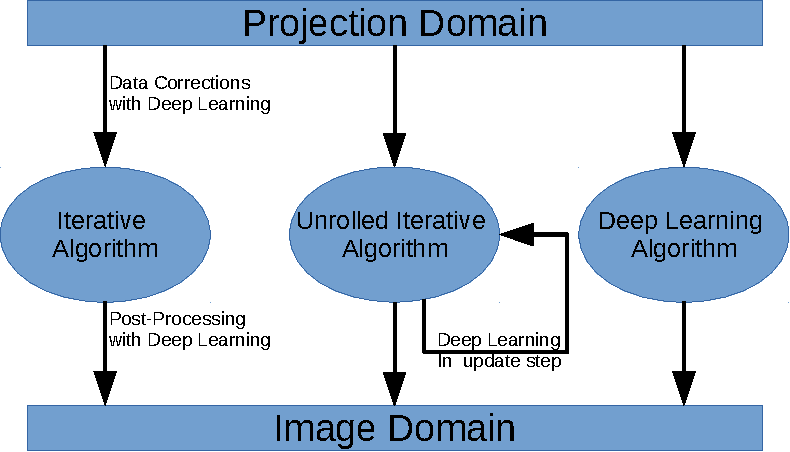
\includegraphics[width=0.8\linewidth]{./Figures/dl_mi.pdf}
	\caption{Deep Learning in Medical Image Reconstruction}
	\label{fig:dl}
\end{figure}


Each of these categories are discussed along with reference to existing state of the art methods for \ac{CT} and \ac{PET} image reconstruction in this chapter. 

\section{Data Corrections or Post-processing}

The use of deep learning for the development of either data corrections or post-reconstruction  image based approaches has shown potential to improve the quality of reconstructed images. While it is possible to train a \ac{CNN} to regress directly from the measurement (raw data) domain to the image domain, the use of \ac{CNN} entirely in one particular domain makes it fast and relatively easy to implement. The motivation behind using deep learning architectures for these processing task is the extremely well documented performance in denoising and super resolution tasks. Data corrections involve improving the measurement data either though denoising or finding missing projection angle data. Post-processing in the image domain on the other hand consists of improving images reconstructed with standard reconstruction methods. 
Corrections in measured data $\boldy$ can be expressed as finding an estimate $\boldyhat$ through a neural network $F$ with parameters $\bm{\theta}$. 
\begin{equation}\label{eq:data_cor}
	\boldyhat = \bm{F}_{\bm{\theta}} (\boldy)
\end{equation} 
The new set of corrected data $\boldyhat$ are then used to reconstruct images through traditional methods. An example of data corrections in \ac{PET} image reconstruction through sinogram repair is proposed by \cite{whiteley2019cnn}, where a \ac{CNN} is utilized to predict missing projection data for total body \ac{PET} image reconstruction. The repaired sinograms eventually improve image reconstruction by standard methods.

In \ac{CT} imaging, missing projection data in sparse-view setting is estimated through neural networks. An example in this regard is proposed in \cite{lee2018deep}, where the authors use U-Net to map sparse-view sinograms to full-view sinograms and then reconstruct the images using \ac{FBP}. Another idea to improve the raw data through scatter correction is proposed in \cite{maier2018deep}. In this work a modified U-Net is used to estimate scatter and correct the raw data in order to improve \ac{CT} images. 

Improvements in the images reconstructed by traditional methods are usually brought about through neural networks designed for denoising or super resolution. An image $\boldxhat$ ($\boldlambdahat$ or $\boldmuhat$) estimated by conventional methods like \ac{FBP} or \ac{OSEM} is improved through a neural network:

\begin{equation}\label{eq:post_pro}
\boldx_{\mathrm{den}} = \bm{F}_{\bm{\theta}} (\boldxhat)
\end{equation} 
where $\boldx_{\mathrm{den}}$ is the post-processed image. Over the years the trend in \ac{PET} imaging has been towards reducing the dose of the radiotracer injected into the patient, which in turn leads to noisier reconstructed images. The approach has been to create datasets with conventional algorithms (like \ac{OSEM}) for both low-dose and normal dose settings and then train a neural network to achieve normal dose quality starting from low-dose images. Apart from the low dose noise problem, in \ac{CT}, improvements in sparse-view imaging through has been an active area of research. The focus here is to reduce the artifacts produced by \ac{FBP} with sparse-view sinograms. These artifacts are either removed by first finding the missing projections and repairing the sinograms or by post-processing the images. In both these scenarios \ac{FBP} is utilized; in the former case neural network corrects the sinograms thereby providing full-view sinograms for reconstruction and in the latter case \ac{FBP} estimated artifact effected images are improved by the neural network.  

Some of the recent developments in post-processing and data corrections for \ac{PET} and \ac{CT} are summarized in Table~\ref{table:pp_PET} and Table~\ref{table:pp_CT}. A short description of the method along with the citation is given in the second column of both the tables. These approaches typically modify an existing neural network architecture to suit the problem they are addressing. U-Net is one of the most utilized architectures as seen in the third column where the base neural network is given. The datasets utilized by each of these is works is mentioned in the final column. Along with proposed modifications of established neural networks, these approaches typically use loss functions consisting of multiple components. The authors in \cite{gong2018pet} used perceptual loss along with \ac{MSE} to preserve qualitative and quantitative accuracy of the reconstructed images. The work proposed by \cite{whiteley2020fastpet} uses \ac{MSSIM} along with perceptual loss and \ac{MAE}. Another strategy used is pre-training on simulated data followed by fine-tuning on real patient data. Data corrections in the form of scatter correction of the sinogram data is proposed in \cite{qian2017deep}. The authors use \ac{CNN} followed by \ac{FC} layers in their approach. In \ac{CT} imaging there are works that do denoising of low-dose sinograms (\cite{ma2021sinogram,zhu2020low}) and also finding the missing projections in sparse-view sinograms (\cite{lee2018deep}). The same problem is tackled in the image domain through denoising (\cite{yang2018low}) and artifact removal for sparse-view problem (\cite{jin2017deep,xie2018artifact,zhang2018sparse}).
\begin{table}[ht!]
	\centering
	\caption{Summary of recent works on data corrections and post-processing approaches in \ac{PET}}
	\label{table:pp_PET}
	\scriptsize
	\begin{tabular}{||c|c|c|c||} 
		\hline
		Sl.No.    & Method             & Base Neural  & Dataset        \\ %[0.5ex] 
		          &                    &  Network     &                \\
		\hline\hline
		1         & \cite{gong2018pet} & \ac{CNN} with residual & BrainWeb and XCAT  \\     
		          &  Low-dose Image    &  blocks                & phantoms; Fine-tuning/testing  \\ 
		          &   Denoising        & & with real patient data       \\ 
		\hline
		2         &  \cite{whiteley2020fastpet}& U-Net with residual & Real PET/CT data \\
		          & Histo Image        & blocks      &        \\
		          & Correction         &                &        \\
		\hline  
		3         & \cite{zhao2020study}& Cycle GAN    & Real PET/CT data  \\ 
       	          & Low-dose Image      &              &                   \\ 
       	          & Denoising           &              &                   \\ 
       	\hline
       	4         & \cite{qian2017deep} & CNN with fully    & Monte Carlo simulations  \\ 
                  & Sinogram Scatter    & connected layer   & with phantoms            \\ 
       	          & Correction          &                   &                          \\ 
       	\hline
       	5         & \cite{hong2018enhancing}& Deep residual CNN & Digital phantoms  \\ 
       	          & Single Image Super      &                   &             \\ 
       	          & Resolution for sinograms&                   &                          \\ 
       	\hline
       	6         & \cite{sanaat2021deeptofsino}&   ResNet       & Real TOF-PET/CT data  \\ 
       	          & Low-dose to full-dose    &                   &             \\ 
       	          & sinogram synthesis    &                      &                          \\ 
       	\hline
       	
	\end{tabular}
	
\end{table}

\begin{table}[ht!]
	\centering
	\caption{Summary of recent works on data corrections and post-processing approaches in \ac{CT}}
	\label{table:pp_CT}
	%\footnotesize
	\scriptsize
	\begin{tabular}{||c|c|c|c||} 
		\hline
		Sl.No.    &       Method             & Base Neural          & Dataset        \\ %[0.5ex] 
            	  &                          &    Network                      &                \\
		\hline\hline
		1         & \cite{lee2018deep}       &   Residual U-Net     & Simulated projections          \\     
		          &  Sinogram synthesis      &                      & from real patient data         \\ 
		          &   for sparse-view CT     &                      &                                \\ 
		\hline
		2         &  \cite{jin2017deep}      & Residual U-Net       & Phantom and Real patient       \\
		          & Artifact removal in      &                      &   data along with projections  \\
		          & sparse-view reconstructed images&               &                                \\
		\hline  
		3         & \cite{xie2018artifact}   & Improved GoogleNet   & Simulated projections          \\ 
		          & Artifact removal in      &                      & from real data                 \\ 
		          & sparse-view reconstructed images&               &                                \\ 
		\hline
		4         & \cite{zhang2018sparse}    & DeneNet with        & Simulated projections          \\ 
		          & Artifact removal in       & deconvolutions      & from real data                 \\ 
		          & sparse-view reconstructed images&               &                                \\ 
		\hline
		5         & \cite{ma2021sinogram}     & Attention residual  & Real data along with           \\ 
		          & Low dose sinogram         &  dense CNN          & projections                    \\ 
		          & denoising                 &                     &                                \\ 
		\hline
		6         & \cite{yang2018low}        &    Wasserstein-GAN & Real data along with            \\ 
		          & Low-dose image            &                    & projections                     \\ 
		          & denosing                  &                    &                                 \\ 
		\hline
		7         & \cite{zhu2020low}         &  Three-segment network  & Real data along with            \\ 
		          & Simultaneous sinogram and &  ADAPTIVE-NET      & projections                     \\ 
	 	          & image domain denoising    &                    &                                 \\ 
		\hline
		
	\end{tabular}
	
\end{table}

An important aspect of the methods discussed in this section is that they all claim to provide fast reconstructed images using well established neural network architectures. This also stems from the fact that most of these approaches start with an image estimate that is also obtained with a relatively faster conventional method, like \ac{FBP} for \ac{CT} and \ac{OSEM} for \ac{PET}. These fast estimates are usually very noisy or artifact ridden. These approaches rely on the neural network to handle the noise and artifacts. The attractiveness of these methods is the simplicity, ease of implementation and the lack of requirement of large datasets of raw detector data. 

\section{Hybrid Methods}

The methods mentioned in this section and the next, are directly involved in the reconstruction process, rather than being exclusive to data corrections or post-reconstruction processing. The hybrid methodology for image reconstruction combines model-based and neural network approaches exploring the benefits of both methods. In this section we discuss some of the recent works in both \ac{PET} and \ac{CT} that fall in the category of hybrid methods.

\begin{itemize}


\item Data-driven information learned by a neural networks can be incorporated into an iterative algorithm through the regularization term. \cite{gong2019iterative} used a modified version of the U-Net comprising of multi-channel input to represent \ac{PET} images.
\begin{equation}\label{eq:iter_CNN}
\boldlambda = \bm{F}_{\bm{\theta_{\mathrm{fixed}}}}(\bm{z})
\end{equation} 
where $\bm{F}_{\bm{\theta_{\mathrm{fixed}}}}$ represents the trained denoising neural network (modified U-Net) with fixed trainable parameters $\theta_{\mathrm{fixed}}$. The \ac{PET} reconstruction model (from \ref{eq:PET}) can be modified to incorporate \ref{eq:iter_CNN}. 

\begin{equation}\label{eq:mod_PET}
	\boldybar(\boldlambda) = \boldA \bm{F}_{\bm{\theta_{\mathrm{fixed}}}}(\bm{z}) + \bm{r}
\end{equation}
The unknown image $\boldlambda$ can be estimated using the maximum likelihood criterion:
\begin{equation}\label{eq:iter_CNN2}
\boldlambdahat = \bm{F}_{\bm{\theta_{\mathrm{fixed}}}}(\bm{\hat{z}})
\end{equation} 
\begin{equation}
\boldlambdahat=\underset{\boldlambda \ge 0}{\operatorname{argmin}} \; L(\bm{z})
\end{equation}

In order to ease the difficulty of solving the above due to the non-linearity of the neural network, the authors adapted a constrained version of the above:

\begin{equation}\label{constr}
 	\operatorname{max} \; L(\bm{\boldlambda});  \; \mathrm{s.t.} \; \boldlambda = \bm{F}_{\bm{\theta_{\mathrm{fixed}}}}(\bm{\hat{z}})
\end{equation}
To solve the above optimization problem the authors used the augmented Lagrangian format:
\begin{equation}
L_{\rho}=L(\boldlambda)-\frac{\rho}{2}\|\boldlambda-\bm{F}_{\bm{\theta_{\mathrm{fixed}}}}(\bm{z})+\bm{\gamma}\|^{2}+\frac{\rho}{2}\|\bm{\gamma}\|^{2},
\end{equation}
The authors used the \ac{ADMM} algorithm to split the above into three steps:

\begin{equation}\label{eq:ad1}
\boldlambda^{N+1}=\underset{\boldlambda}{\arg \max} \; L(\boldlambda)-\frac{\rho}{2}\left\|\boldlambda-\bm{F}_{\bm{\theta_{\mathrm{fixed}}}}(\bm{z})^{N}+\bm{\gamma}^{N}\right\|^{2}
\end{equation}

\begin{equation}\label{eq:ad2}
\bm{z}^{N+1}=\arg \min \left\|\bm{F}_{\bm{\theta_{\mathrm{fixed}}}}(\bm{z})-\left(\boldlambda^{N+1}+\bm{\gamma}^{N}\right)\right\|^{2}
\end{equation}

\begin{equation}\label{eq:ad3}
\bm{\gamma}^{N+1}=\bm{\gamma}^{N}+\boldlambda^{N+1}-\bm{F}_{\bm{\theta_{\mathrm{fixed}}}}(\bm{z})^{N+1}
\end{equation}
\ref{eq:ad1} is equivalent to penalized \ac{PET} reconstruction and the authors used the optimization transfer method proposed in \cite{wang2012penalized}. The second part of the algorithm (from \ref{eq:ad2}) involving the input $\bm{z}$ update, is a non-linear version of the least squares problem. In the above methodology, the network parameters $\bm{\theta}$ are fixed while the input to the network $\bm{z}$ is updated. The authors extended this approach in \cite{gong2018pet2} by using a fixed input to the network $\bm{z}_{\mathrm{fixed}}$, while setting the network parameters to update. The fixed input to the network was an MRI image while the network training was based on the concept of deep image prior (\cite{ulyanov2018deep}). The second sub-problem was modified to reflect the update in the network parameters:

\begin{equation}\label{eq:dip}
\bm{\theta}^{N+1}=\arg \min \left\|\bm{F}_{\bm{\theta}}(\bm{z_{fixed}})-\left(\boldlambda^{N+1}+\bm{\gamma}^{N}\right)\right\|^{2}
\end{equation}

Both these methods require that the raw data also agree with the denoising \ac{CNN}. The images reconstructed are reported to have better lesion contrast compared to the post-processing \ac{CNN} denoising approaches, indicating an advantage of the hybrid methods, despite being slightly tedious to implement and having longer prediction times.

\item Apart from using neural networks for regularization, the prior information captured by them can be combined with established model-based methods. One such approach called FBSEM-Net was proposed by \cite{mehranian2020model}. Their unrolled method is based on forward-backward splitting (FBS) algorithm. The objective function for their method was:

\begin{equation}
\boldlambda^{N}=\underset{\boldlambda}{\operatorname{argmax}}\left\{L(\boldlambda \mid \boldy)-\frac{1}{2 \beta}\left\|\boldlambda-\boldlambda_{R e g}^{N}\right\|^{2}\right\}
\end{equation}
with $\beta$ being a hyper-parameter that controls the balance between the data fidelity term and the regularization term. The authors solved the above through the method of separable surrogates proposed in \cite{depierro1995}. The three steps involved in obtaining the final image update: computing the regularization term, finding the EM update and fusing the EM update with the neural network estimated prior. The first step to compute the regularization term cn be written as:

\begin{equation}\label{eq:fbs1}
\boldlambda_{reg}^N = \bm{F}(\boldlambda^{N-1})
\end{equation} 
where $F$ is a residual neural network estimating the regularization term based on the image from the previous iteration. 
The second step involved getting the EM update $\boldlambda_{EM}^{N}$ similar to \ref{eq:mlem}. Finally the image is estimated by
\begin{equation}\label{eq:fb2}
\begin{array}{l}
\lambda_j^{N+1} 
=\frac{2 \lambda_{E M}^{N}}{\left(1-\delta_{j} \lambda_{j, R e g}^{N}\right)+\sqrt{\left(1-\delta_{j} \lambda_{j, R e g}^{n}\right)^{2}+4 \delta_{j} \lambda_{j, E M}^{n}}} ,\; \delta_{j}=\frac{1}{\beta s_{j}}
\end{array}
\end{equation}

During the network training, two reconstructions occur simultaneously, one with good quality reference data and the other with noisy data. The role of the neural network is to denoise the current estimate, such that the fused combined image using \ref{eq:fb2} best agrees with the high quality \ac{MLEM} reconstructed image. The overall methodology constitutes of a very deep network with each iteration being a block of \ac{CNN} along with the conventional \ac{MLEM} layers. 


\item \cite{adler2018learned} proposed a learned primal-dual algorithm which was one of the first methods that combined \ac{MBIR} methods with deep learning for low-dose \ac{CT} image reconstruction. The authors proposed a generalized algorithm that could be modified for other tomographic imaging modalities also. \acp{CNN} are used both in the image domain and the sinogram domain, connected through the forward projection operator and it's adjoint. In many \ac{MBIR} approaches, non-smooth regularizers are used. They are typically handled through smooth approximations which lead to additional parameters and non-exact solutions. As an alternative, proximal methods are used to tackle the non-smooth objective functions. Inspired from one such proximal \ac{PDHG} algorithm (\cite{chambolle2011first}), the authors proposed a learned reconstruction scheme. They replaced the proximal operators with learned parameterized operators (\acp{CNN}) to result in a learned reconstruction operator. The primal and dual operators were parameterized as \acp{CNN} consisting of 3 layers and in total of 64 intermediate convolution channels. The algorithm is summarized in \ref{alg:pd}. 

\begin{algorithm}
	\SetAlgoLined
	For primal and dual variables $x \in X^{N_{primal}}$ and $h \in X^{N_{dual}}$, proximal dual and primal operators represented by neural networks,  $\Gamma_{\theta_{k}^{d}}$, $\Lambda_{\theta_{k}^{p}}$, K iterations,measurement data $\boldy$
	\For{k = 1,2,\dots, K}{
		$\bm{h}^{[k]}=\Gamma_{\theta_{k}^{d}}\left(\bm{h}^{[k-1]}, \bm{A}\left(\boldx_{(2)}^{[k-1]}\right), \boldy\right)$
		
		$\boldx^{[k]}=\Lambda_{\theta_{k}^{p}}\left(\boldx^{[k-1]},\left[\bm{A}\left(\boldx_{(1)}^{[k-1]}\right)\right]^{*}\left(\bm{h}_{(1)}^{[m]}\right)\right)$
				
	}
    \Return $\boldxhat = \boldx_{(1)}^{[K]}$
	\caption{Learned Primal-Dual}
	\label{alg:pd}
\end{algorithm}

The neural networks and the projection/back-projection operators were implemented using operator discretization library (ODL) and Tensorflow \cite{abadi2016tensorflow}. The authors tested their approach on ellipse phantoms and real patient data. They reported better qualitative and quantitative results when compared to TV and deep learning-based post-processing method. 

\item A hybrid method for sparse-view \ac{CT} was proposed in \cite{wu2021drone}. The authors propose a three-stage reconstruction framework consisting of embedding, refinement and awareness. The first module extends the sinogram and reduces the sparse-view artifacts. The refinement part of the method recovers finer details in the images and finally the last module regularizes the images from the earlier modules by ensuring consistency between the measurement data and images. The last module adapted from compressed sensing ensures stability and generalizability in the reconstructed images through a compressed sensing model. The embedding module consists of two neural networks $F_1$ and $F_2$, the first one is a U-Net that operates in the sinogram domain mapping from 60 views to 180 views, and the second one a W-GAN that operates in the image domain refining the image obtained though \ac{FBP} on the upsampled sinograms. It can be represented as follows:

\begin{equation}
\boldx^{\prime}=F_{2}(\bm{A_{2}}^{+}(F_{1} (\boldy)))
\end{equation}
where $\boldx^{\prime}$ is the image estimated by the embedding module, $\bm{A_2}^{+}$ is the \ac{FBP} reconstruction operator for the up-sampled views ($180$). The next module maintains a balance between the extension of views and refining the subsequent details in the images through two neural networks similar to the ones in the first module. The residual between the image predicted by the embedding module and the re-sampled sinogram can be written as: $(\boldy'-\boldA_{2} \boldx')$. The first neural network is trained to minimize the \ac{MSE} between the measurement data labels and predictions.   

\begin{equation}
	\boldy'' = F_3(\boldy'-\boldA_{2} \boldx')
\end{equation} 
The second neural network in the refinement module is trained to minimize the \ac{MSE} between the image data and labels resulting in a refined image:

\begin{equation}
\boldx'' = F_4(\boldA_{2}^{+}(\boldy''))
\end{equation} 
The measurement data and the images are then updated with the predictions from the trained networks:

\begin{equation}
	\boldy^d = \boldy'' + \bm{A_{2}} \boldx' 
\end{equation}

\begin{equation}
    \boldx^d = \boldx' + \boldx''
\end{equation}

\end{itemize}

The final module combines the deep learning-based data image priors ${\boldy^d,\boldx^d}$ and the compressed sensing framework to arrive at an objective function as follows:

\begin{equation}\label{eq:cs}
\min _{\boldx}\left\{\begin{array}{l}
\frac{1}{2}\left\|\mathbf{y}-\mathbf{A}_{1} \boldx \right\|^{2}+\frac{\alpha_{1}}{2}\left\|\boldy^{d}-\mathbf{A}_{2} \boldx\right\|^{2} \\
+\frac{\alpha_{2}}{2} \mathrm{~W} \boldx+\frac{\alpha_{3}}{2} \mathrm{~W}\left(\boldx-\boldx^{d}\right)
\end{array}\right\}
\end{equation}
where $\alpha_{1} \ge 0$ balances the two data fidelity terms, $\boldA_{1}$ represents the system matrix that projects the lower-sampled data (60 views) and $\boldA_{2}$ represents the system matrix that projects the higher up-sampled data ($180 views$). For the regularization the authors used a variation of TV, called total difference represented by $W$. $\alpha_{2}$ and $\alpha_{3}$ are the regularization hyper-parameters. The authors validated their method on clinical and pre-clinical datasets and reported superior performance of their proposed method when compared to deep learning-based methods like FBPConvNet (\cite{jin2017deep}), HD-Net (\cite{wu2020high}) and DL-PICCS (\cite{zhang2020deep}).
 
Other works in the hybrid approach include the article by \cite{xie2019generative}, who extended \cite{gong2019iterative} by replacing the U-Net with a \ac{GAN} for image representation within the iterative framework. \cite{kim2018penalized} incorporated a trained denoising convolutional neural network (DnCNN) along with a novel local linear fitting function into the iterative algorithm. The DnCNN which is trained on data with multiple noise levels improves the image estimate at each iteration. They used simulated and real patient data in their study. In \cite{gupta2018cnn}, a U-Net is used to encode the prior, i.e., to project the current estimate to the prior image set while gradient descent enforces measurement consistency. The drawbacks of the methods described in this section are the slow reconstruction time and high computational expense, since the optimization procedure is carried out also during test time. Despite the advantage of producing state of the art results (\cite{reader2020deep,leuschner2021quantitative}) along with the stability and consistency offered by these hybrid methods, the justification of complexity vs accuracy trade-off is still a topic of active research. 


\section{Direct Reconstruction with Deep Learning}

The third approach is using deep learning-based methods to directly map from projection to image space. Essentially neural network can be modeled to approximately learn  the inverse mapping from measurement ($\boldy$) to image ($\boldx$). A neural network ($F$) with trainable parameters ($\theta$) can be represented as:

\begin{equation}\label{eq:direct}
\boldxhat=F_{\bm{\theta}}(\boldy)
\end{equation}
where $\boldxhat$ is the reconstructed image estimated by the neural network. Once trained, the reconstructed images are estimated by a single pass though the network, making it the fasted approach for image reconstruction. However, the challenges include the management of data, the large number of training parameters and stability at testing time. Due to these challenges, this approach has been less explored compared to the two approaches discussed above. 

The deep learning architecture proposed by \cite{zhu2018image} called AUTOMAP uses \ac{FC} layers (which encode the raw data information) followed with convolutional layers. The first three layers in this architecture are \ac{FC} layers with dimensions $2n^2$,$n^2$ and $n^2$ respectively where $n\times{}n$ is the dimension of the input image. The AUTOMAP requires the estimation of a huge number of parameters which makes it computationally intensive. Although initially developed for \ac{MRI}, AUTOMAP has been claimed to work on other imaging modalities too. Brain images encoded into sensor-domain sampling strategies with varying levels of additive white Gaussian noise were reconstructed with AUTOMAP.  Within the same concept of using \ac{FC} layers' architectures a three stage image reconstruction pipeline called DirectPET has been proposed to reduce associated computational issues  \cite{whiteley2019direct}. The first stage down-samples the sinogram data, following which a unique Radon transform layer encodes the transformation from sinogram to image space. Finally the estimated image is improved using a super resolution block. This work was applied to full body \ac{PET} images and remains the only approach that can reconstruct multiple slices simultaneously (up to 16 images). DeepPET is another approach implemented on simulated images using \ac{CED} architecture based on the neural network proposed by the visual geometric group \cite{haeggstroem2018deeprec}. Using realistic simulated data, they demonstrated a network that could reconstruct images faster, and with an image quality (in terms of root mean squared error) comparable to that of conventional iterative reconstruction techniques. \cite{liu2019deep} proposed a direct conditional \ac{GAN} based approach, that replaced the \ac{CED} with a U-Net.    


For direct \ac{CT} image reconstruction, \cite{li2019learning} proposed an architecture termed iCT-Net consisting of $12$ layers that are a combination of convolutions and modified fully-connected layers. The $12$ layers are separated into segments and are trained separately before being combined for end-to-end training. To reduce the number of parameters in learning the mapping for full resolution \ac{CT} reconstruction, \cite{fu2019hierarchical} proposed a breakdown of the problem into smaller fragments that can be mapped onto a hierarchical network architecture. The approach proposed in \cite{ye2018deep} converts the sinogram data into a stack of back projections for each angle, which are then fed into a \ac{CNN}. The spatial in-variance of the \ac{CNN} is exploited to learn the mapping from these single view stacked back projections onto reconstructed images. Currently, we observe that adversarial networks are increasingly used in scenarios with high-resolution images. In \cite{thaler2018sparse} a Wasserstein generative adversarial network \cite{arjovsky2017wasserstein} is proposed for sparse-view \ac{CT} image reconstruction. The authors used a combination of $L_1$ loss and adversarial loss to train their network. The generator in their work is a U-Net and the discriminator a typical classification \ac{CNN}. It is to be noted that the authors performed their experiments on down-sampled images of resolution $128\times 128$. 




